
\cleardoublepage


\chapter{Experimental Validation}

% other stuff
% ------------------------------------------------------------

\section{Experimental Procedures}


\subsection{Gold Foil Tube}

% foils were individually weighed and included in table
First, the foils were individually weighted and those values are shown in \TAB{tab:au_masses}.
% the device was assembled
The device was then assembled as described in the modeling section.
% outer shielding was removed from the beam port configuration
Some of the outer shielding around the beam port was removed to access the collimator.
% the devices was attempted to fit into the beam port but deformation prevented insertion
Initially, an attempt was made to insert the device into the collimator, but deformation in the aluminum portion of the collimator prevented insertion.
% the device was ground down to fit in and inserted to where the first piece was in line with the aperture of the collimator
The first few inches of the device were then ground down with a belt sander to reduce the diameter of the device slightly.
The device was then inserted into the reactor.
% then, the reactor was powered on to __ kwth
Reactor power was brought to 100kW(th).
% the reactor remained at power for __ hours
The reactor remained at power for approximately 2.5 hours.
% then the reactor was shut down
Following the irradiation, the reactor was shut down.
% after allowing the device to cool for a bit, the individual foils were removed and bagged
A cooling period was necessary for the short-lived isotopes produced in the collimator and device to decay.
Then, the device was removed, and from the device, the individual foils were removed and bagged.
% foils were moved to an individual counting station where they were counted (gamma spec)
The foils were moved to an individual counting station, where they were sequentially counted using an HPGE.

% foil tube experimental configuration
\begin{figure}[htb]
\centering
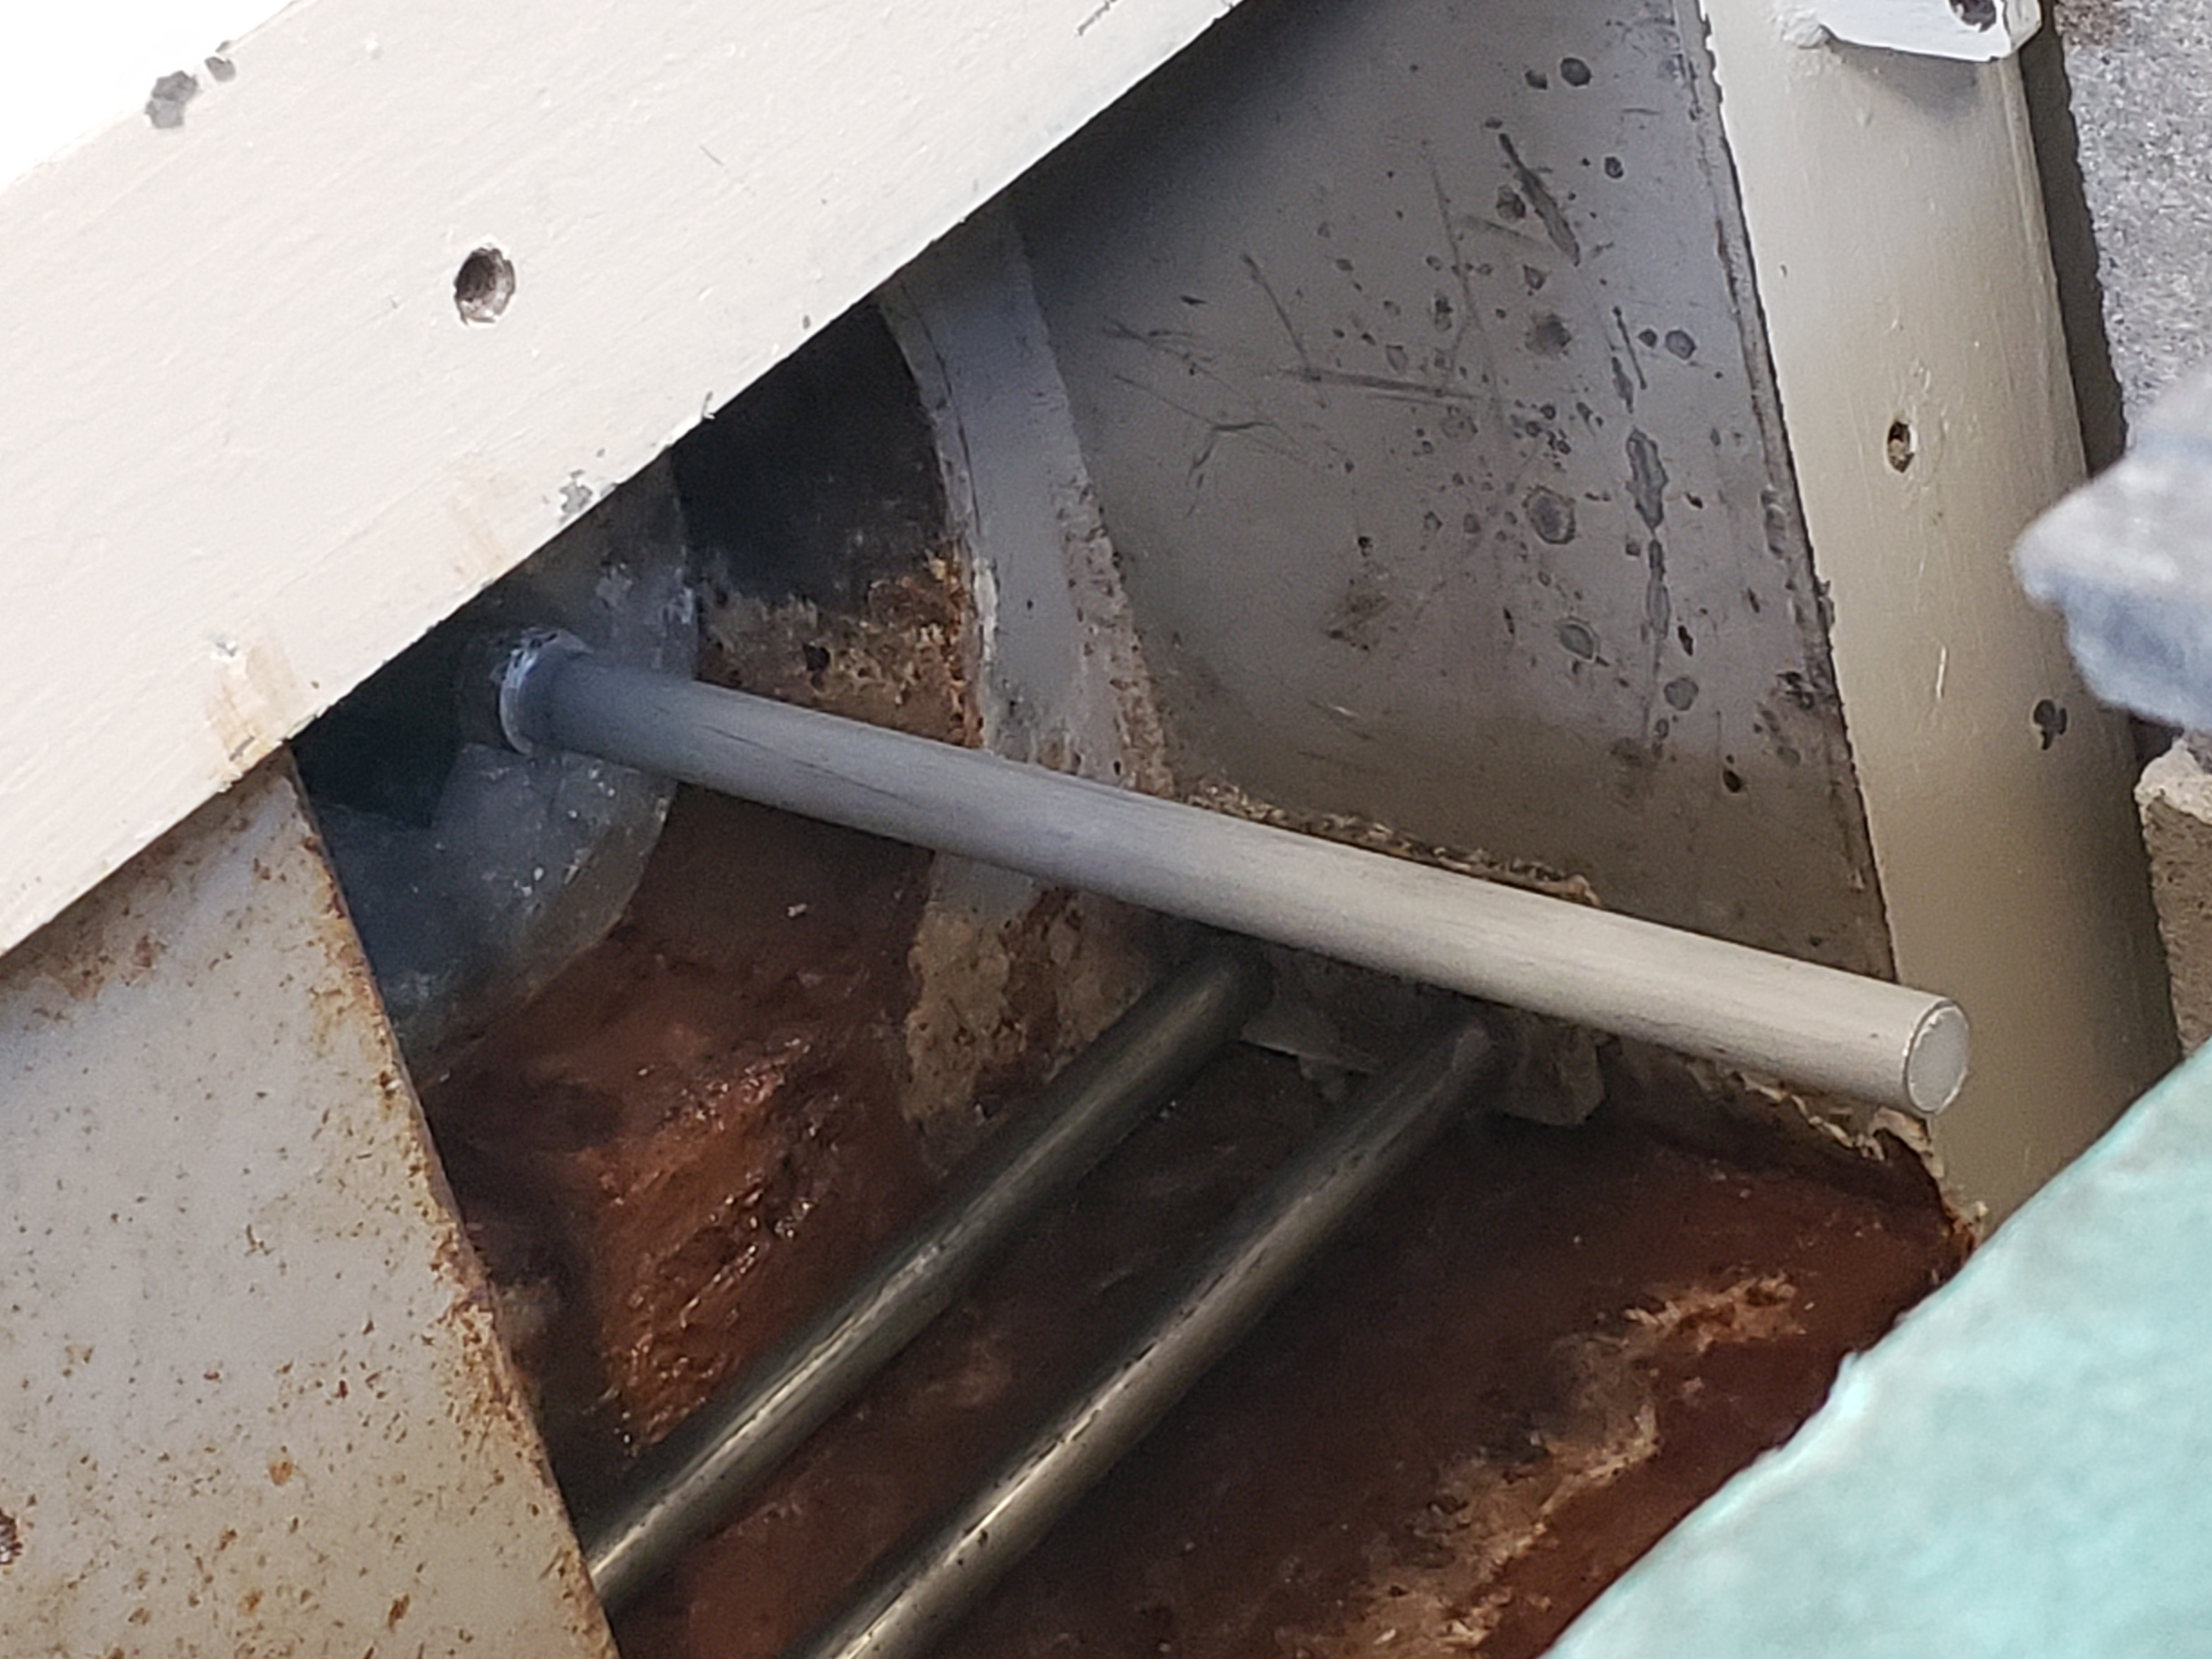
\includegraphics[height=3in]{tex/figures/ft_au_in_beam.jpg}
\caption[Gold Foil Tube Experiment]{A view of the gold foil tube inserted into the NEBP collimator.}
\label{fig:ft_au_in_beam}
\end{figure}

% this contains all of the advantg parameters
\begin{table}[h]\centering
\label{tab:au_masses}
\caption{The masses of the gold foils.}
\begin{tabular}{ r | r | l }
\toprule
Foil ID  & Position (in.)     &   Foil Mass (g)\\
2 & 0 & 0.0320\\
13 & 1 & 0.0312\\
4 & 2 & 0.0320\\
5 & 3 & 0.0318\\
6 & 4 & 0.0319\\
7 & 5 & 0.0325\\
8 & 6 & 0.0326\\
9 & 7 & 0.0320\\
10 & 8 & 0.0318\\
11 & 9 & 0.0326\\
12 & 10 & 0.0317\\
\end{tabular}
\end{table}

\subsection{Bonner Sphere Spectrometer}

% for the bonner spheres, the device was placed vertically in a manner that aligned the detection crystal with the beam at a distance of ___ cm
For the BSS irradiation, the device was positioned vertically in a manner that aligned the detection crystal with the center of the beam at a distance of (???) cm.
% the detector was set to aquire for __ s, and then the reactor was brought to __ kwth.
The detector was set to aquire for 300 s live time and then the reactor was brought to 100kW(th).
% the lld setting was adjusted to where the noise could be removed, but the lithium,T peak wasn't affected
The lld setting was electronically adjusted to reduce the detector dead time, without removing the $^6$Li(n,t) peak.
% spectra were aquired for each configuration
Spectra were aquired for the bare, 2", 3", 5", 8", 10", and 12" configurations.
For the 12" sphere, a live time of 600 seconds was used to help achieve lower counting statistics.
% the reactor was then powered off
Following the experiment, the reactor was powered off.

% ------------
% i need to put all the detection settings and stuff here
% ------------


% ------------
% also, add pictures of both setups
% ------------

% ------------------------------------------------------------
% other stuff
